\documentclass{standalone}
\usepackage{tikz}

\begin{document}

% description: multiple arrows on a single path
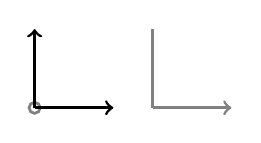
\begin{tikzpicture}[line width=1pt]
\draw[gray] (0,0) circle [radius=2pt];
\draw (0,0) 

% start
% relative coordinate, 
% without changing current position
	edge [->] +(0,1) 
	edge [->] +(1,0)
;

% counterexample, only draws one arrow
	\draw [gray]
		(1.5,0) [->] -- +(0,1)
		(1.5,0) [->] -- +(1,0);

% end

\end{tikzpicture}

\end{document}
